%%%%%%%%%%%%%%%%%%%%%%%%%%%%%%%
%                             %
% Luther Michaels             % 
% ECE 351-52                  %
% Lab 2                       %
% September 16, 2021          %
% User-Defined Functions      %
%             Lab Report      %
%                             %
%%%%%%%%%%%%%%%%%%%%%%%%%%%%%%%

%%%%%%%%%%%%%%%%%%%%%%%%%%%%%%%%%%%%%%%%%%%
%%% DOCUMENT PREAMBLE %%%
\documentclass[12pt]{report}
\usepackage[english]{babel}
\usepackage{url}
\usepackage[utf8x]{inputenc}
\usepackage{amsmath}
\usepackage{graphicx}
\graphicspath{{images/}}
\usepackage{parskip}
\usepackage{fancyhdr}
\usepackage{vmargin}
\usepackage{listings}
\usepackage{hyperref}
\usepackage{xcolor}

\definecolor{codegreen}{rgb}{0,0.6,0}
\definecolor{codegray}{rgb}{0.5,0.5,0.5}
\definecolor{codeblue}{rgb}{0,0,0.95}
\definecolor{backcolour}{rgb}{0.95,0.95,0.92}

\lstdefinestyle{mystyle}{
    backgroundcolor=\color{backcolour},   
    commentstyle=\color{codegreen},
    keywordstyle=\color{codeblue},
    numberstyle=\tiny\color{codegray},
    stringstyle=\color{codegreen},
    basicstyle=\ttfamily\footnotesize,
    breakatwhitespace=false,         
    breaklines=true,                 
    captionpos=b,                    
    keepspaces=true,                 
    numbers=left,                    
    numbersep=5pt,                  
    showspaces=false,                
    showstringspaces=false,
    showtabs=false,                  
    tabsize=2
}
 
\lstset{style=mystyle}

\setmarginsrb{3 cm}{2.5 cm}{3 cm}{2.5 cm}{1 cm}{1.5 cm}{1 cm}{1.5 cm}

\title{2}	% Title						
\author{Luther Michaels}	% Author		
\date{September 16, 2021}   % Date

\makeatletter
\let\thetitle\@title
\let\theauthor\@author
\let\thedate\@date
\makeatother

\pagestyle{fancy}
\fancyhf{}
\rhead{\theauthor}
\lhead{\thetitle}
\cfoot{\thepage}
%%%%%%%%%%%%%%%%%%%%%%%%%%%%%%%%%%%%%%%%%%%%

\begin{document}

%%%%%%%%%%%%%%%%%%%%%%%%%%%%%%%%%%%%%%%%%%%%%%%%%%%%%%%%%%%%%%%%%%%%%%%%%%%%%%%%%%
%%% TITLE PAGE %%%
\begin{titlepage}
    \centering
    \vspace*{0.5 cm}

    \begin{center}    
        \textsc{\Large   ECE 351 - Section \#52}\\[2.0 cm]	
    \end{center}  
	\textsc{\Large User-Defined Functions  }\\[0.5 cm]
	\rule{\linewidth}{0.2 mm} \\[0.4 cm]
	{ \huge \bfseries \thetitle}\\
	\rule{\linewidth}{0.2 mm} \\[1.5 cm]
	\begin{minipage}{0.4\textwidth}
		\begin{flushleft} \large
		\end{flushleft}
		\end{minipage}~
	\begin{minipage}{0.4\textwidth}
		\begin{flushright} \large
			\emph{Submitted By:} \\
			Luther Michaels \break
			
			\emph{Submission Date:} \\
			September 16, 2021
		\end{flushright}
	\end{minipage}\\[2 cm]
\end{titlepage}

%%%%%%%%%%%%%%%%%%%%%%%%%%%%%%%%%%%%%%%%%%%%%%%%%%%%%%%%%%%%%%%%%%%%%%%%%%%%%%%%%%
%%% TABLE OF CONTENTS %%%

\tableofcontents
\pagebreak

%%%%%%%%%%%%%%%%%%%%%%%%%%%%%%%%%%%%%%%%%%%%%%%%%%%%%%%%%%%%%%%%%%%%%%%%%%%%%%%%%%
%%% LAB REPORT %%%
\renewcommand{\thesection}{\arabic{section}}
\section{Introduction}

The major focus of exploration for this lab is on user-defined functions. The goal is to learn how to implement these functions in Python. A function will be altered in accordance with the principles of time reversal, time shifting, time scaling, and differentiation in turn to verify their expected effects. \\

Successful execution of the lab procedure relies on a solid understanding of numpy arrays, loops, and conditionals. Numpy arrays are useful for functions since they can store an output at each index; loops allow a series of inputs to be iterated through; and conditionals are the foundation for building many functions. When constructing function plots, the step size should be sufficient to produce an image with good resolution. The plots should include a title, y-axis labels, and a single x-axis label below the lowest subplot. All functions and plots can be produced using Python code written within the Spyder software and hand plots can be made in draw.io. \\

\section{Equations}

\begin{equation}
    y(t)= cos(t)
\end{equation}
\begin{equation}
    u(t)=
    \begin{cases}
    0 & t < 0\\
    1 & t\ge 0\\
    \end{cases}
\end{equation}
\begin{equation}
    r(t)=
    \begin{cases}
    0 & t < 0\\
    t & t\ge 0\\
    \end{cases}
\end{equation}
\begin{equation}
    y(t)= r(t) - r(t - 3) + 5 \cdot u(t - 3) - 2 \cdot u(t - 6) - 2 \cdot r(t - 6)
\end{equation}
\begin{equation}
    m = \Delta y / \Delta t
\end{equation}

\section{Methodology}

Part 1 of the lab outline requested a user-defined function that modelled a cosine as shown in Equation 1. All solutions for this lab utilized the numpy and matplotlib.pyplot Python packages. This function could be simply defined using the included numpy.cos() function. Func1 was written to take a time input variable and return a variable containing the numpy cosine function for the given time. The time interval of 0 to 10s was set using np.arange(), adding the step size to the upper bound so as to include the full sequence. The step size and plotting process were then copied from the good resolution lab example and adjusted to match the function information. \\

\begin{lstlisting}[language=Python]
"""Part 1, Task 2"""
steps = 1e-2    # Step size

def func1(t): # Variable t is sent to the function.
    y = np.cos(t)
    return y # Return y assigned the numpy cosine function.

t = np.arange(0, 10 + steps, steps) # Time interval (0,10)
y = func1(t)

plt.figure(figsize = (10, 7))
plt.subplot(2, 1, 1)
plt.plot(t, y)  # Plot definition
plt.grid()
plt.title('Part 1: Task 2')   # Title
plt.ylabel('y(t) = cos(t)')   # y-axis label
plt.xlabel('t')     # x-axis label
plt.show()
\end{lstlisting}

Part 2 began with the initial task of transferring the provided graph into a function comprised of individual step and ramp functions. The results of this undertaking are shown in Equation 4. The function was found by analyzing the x and y coordinates and slopes of the steps and ramps, then applying the corresponding coefficients and shifts to those functions. The negative ramp function shifted right by 3s is necessary to cancel the ramp from continuing to climb beyond t = 3s. \\

User-defined step and ramp functions were then implemented using loops and conditionals. Each created a variable for a numpy array filled with zeroes. The duration of the time input was then iterated through. An if statement was used such that whenever time at the given index was less than zero, the function variable would be set to zero at that index. For the step function, the else condition would set the variable to 1 at that index as in Equation 2. Alternatively, the ramp would set the variable to the indexed value of time like in Equation 3. \\

The hand-produced equation for the graph in Part 2 could be implemented in Python similarly to the cosine. The function would take a time input variable, and then return a variable assigned with Equation 4. The only adjustment would be to include the names of the step and ramp functions created before. After adding labels, the plot interval could be altered for the new time requirement. 

Part 3 is where several signal operations were tested on the function for Equation 4. The time reversal was implemented by plotting the function with an input of -t for the time variable. In order to view the plot, np.arange() was used to set the time window from -5 to 10s. Likewise, both time shifts were created by simply altering the time input. The first input was t - 4 and the second -t - 4. Again, np.arange() was used to define intervals in which both plots could be properly viewed. The time scaling operations changed the time input to t/2 and 2t respectively. By assigning a variable to the return from these function calls, the desired plot could be formed. \\

The derivative of Equation 4 was found graphically. The solution can be found by recalling that the derivative at each point is the instantaneous slope of the function. If the slope is horizontal, the derivative at that point is equal to 0. A vertical slope indicates that the derivative is undefined or a discontinuity. \\

To define the derivative function in Python, a variable for a numpy array of zeroes was first created. Slope is given as the change in function output divided by the change in t as shown in Equation 5. The difference in output was calculated outside the loop using np.diff() over the function for Equation 4. The difference in time was simply found using np.diff(t). Iterating through all time save the last value, the value of the array at each index is assigned the value of the change in height at that index divided by the change in t. \\

Github Link: \url{https://github.com/Luther-Michaels}

\section{Results}

Below is shown the plot of the cosine function from Part 1 of the lab procedure. The output begins at 1 as expected and repeats every 2$\pi$ s. The smooth curve of the sinusoidal shape suggests that the step size is sufficient to produce good resolution. \\

\begin{center}
    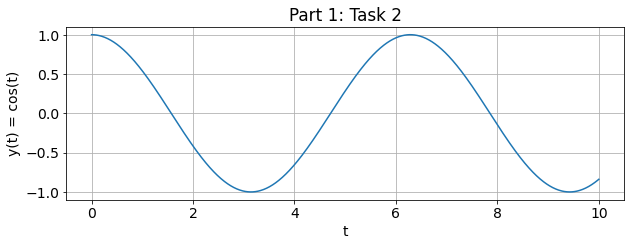
\includegraphics[scale = 0.48]{Lab 2 - Plots/Part1-Task2.png}\\[1.0 cm]
\end{center}

The code for the cosine function in Part 1, Task 2 is provided under Methodology. \\

The user-defined step and ramp functions are shown in the next plot. Both functions remain at 0 for all time less than t = 0s. The step function then jumps to a value of 1 while the ramp obtains the value of t. The results are not perfectly precise, however, as the step function has a slight curve to its vertical leap. Overall, these results align closely with expectations and reflect their function definitions shown in Equations 2 and 3. The title and labels reflect the instructions given for proper plot formatting. \\

\begin{center}
    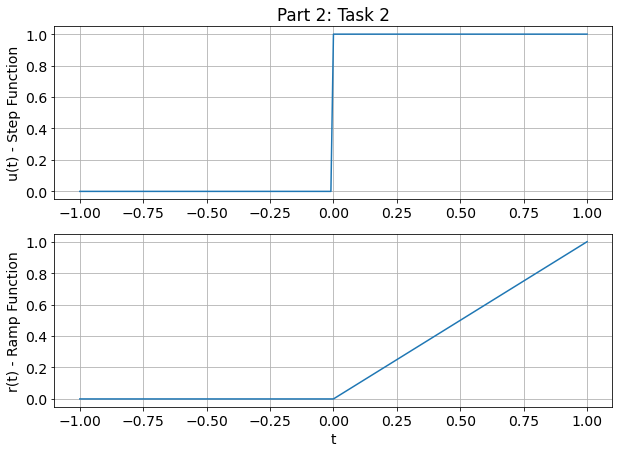
\includegraphics[scale = 0.35]{Lab 2 - Plots/Part2-Task2.png}\\[1.0 cm]
\end{center}

The plot of Equation 4 below matches that of the graph shown in the Part 2 of the lab manual. The ramp increases to 3 from 0 to 3s, steps up to 8, steps down to 6 at 6s, and ramps back down to -2 by 10s. This supports the validity of the handwritten equation as a representation for the graph, as well as the step and ramp functions. \\  

\begin{center}
    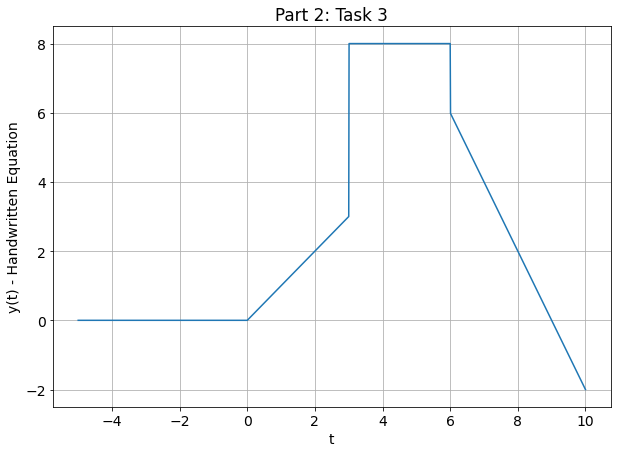
\includegraphics[scale = 0.39]{Lab 2 - Plots/Part2-Task3.png}\\[1.0 cm]
\end{center}

The time reversal of Equation 4 required in Part 3 is given below. As expected, this is a simple revolution around the y-axis. The shape remains the same while all the time coordinates have become negative. An inverse time input responds with an inverted output. \\

\begin{center}
    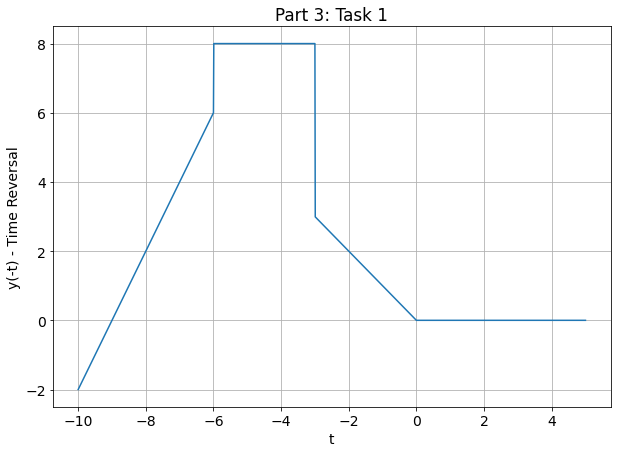
\includegraphics[scale = 0.42]{Lab 2 - Plots/Part3-Task1.png}\\[1.0 cm]
\end{center}

The two time shifts of the equation are shown next. The first has been shifted right by 4s, while the second has moved left by 4s and undergone a time reversal. These results correspond to the outcome we expected from the given inputs. A time shifted input corresponds to an output shifted by the same degree. \\

\begin{center}
    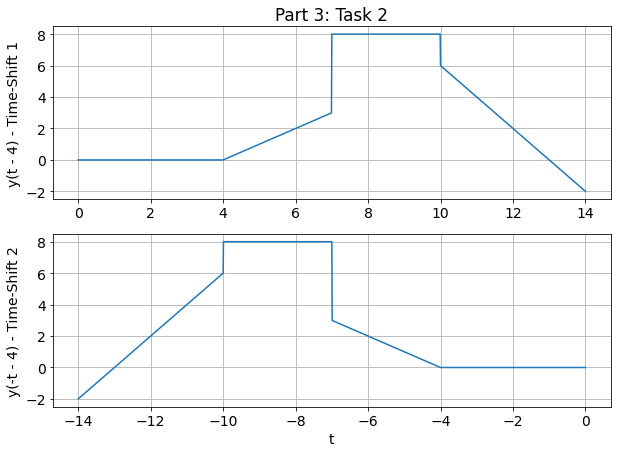
\includegraphics[scale = 0.46]{Lab 2 - Plots/Part3-Task2.png}\\[1.0 cm]
\end{center}

The following plot shows the two time scale operations performed on Equation 4. While the shape remains the same, the time interval each is contained within has been altered. The original time window went from 0 to 10s. The results match what our intuition would suggest. Halving the time input doubles the interval the output covers and doubling the time input halves the output interval. \\

\begin{center}
    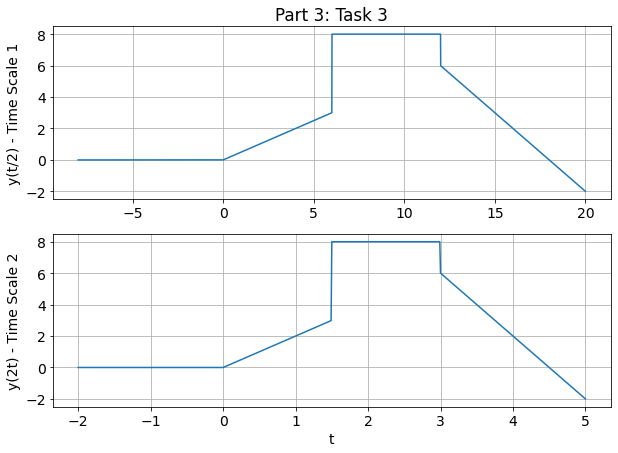
\includegraphics[scale = 0.6]{Lab 2 - Plots/Part3-Task3.png}\\[1.0 cm]
\end{center}

By analyzing the slope of Equation 4, its derivative was mapped out by hand. The following image is a representation of the derivative plotted using draw.io. Instantaneous slope change due to the introduction of a ramp causes a discontinuity. A vertical step function also results in a discontinuity as the slope is undefined. \\

\begin{center}
    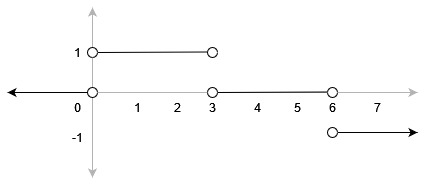
\includegraphics[scale = 0.61]{Lab 2 - Plots/Hand-drawn Derivative.jpg}\\[1.0 cm]
\end{center}

The plot below displays the derivative of Equation 4 plotted using Python. The result is very close to our hand-drawn intuition. The output is 0 before 0s, 1 from 0 to 3s, 0 from 3 to 6s, and -1 beyond. The primary differences are that the Python plot draws the instantaneous slope change at 0s, and also includes the undefined vertical slopes from the step functions. This is typical behavior for a computational graphing software. The Python plot also returns to 0 at 10s. This is due to the fact that there is no subsequent point with which to take a difference calculation. As such, the results closely align with what we would expect. \\

\begin{center}
    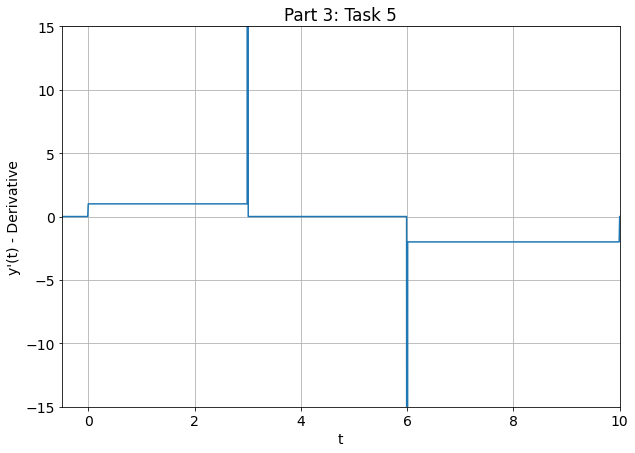
\includegraphics[scale = 0.43]{Lab 2 - Plots/Part3-Task5.png}\\[1.0 cm]
\end{center}

\section{Error Analysis}

I had some difficulty at first in deriving Equation 4 from the graph in Part 2. I realized when attempting to graph it that there was an error somewhere. As the graph continued to ramp up beyond the first step function, I discovered that I had to cancel out that first ramp. Plotting the function again revealed that the adjustments made to the equation were right. \\

I also initially struggled in defining the differentiation function. I realized I needed to take two differences and divide them, but I could not get the differences right. After some reflection, I found that the two differences had to be taken before entering the for loop. Those differences could then be indexed within the loop. \\

\section{Questions}

1. The plots from \textbf{Part 3 Task 4} and \textbf{Part 3 Task 5} are not identical. It is not possible for them to match using the basic plotting functions of the matplotlib.pyplot package. Like many graphing calculators, this is because the method employed to produce a plot is not capable of discovering discontinuities. Consequently, the Python plot will connect two points with a line or run a line towards infinity at these discontinuities. \\

2. The two plots (from \textbf{Part 3 Task 4} and \textbf{Part 3 Task 5}) begin to correlate much less as the step size within the time variable in \textbf{Task 5} increases. This is because the function is sampled much less frequently while the plot still includes part of the infinite discontinuities. It does not identify the peak, but rather still tries to connect a line between points at discontinuities. This means that the discontinuities become more wide and triangular as opposed to the vertical lines present in the \textbf{Task 5} plot. The result is that the differences between the graphs are accentuated. \\

3. The lab tasks, expectations, and deliverables are all clearly communicated. \\

\section{Conclusion}

In this lab we learned to define functions in Python and observed the consequences of several time input adjustments. We developed an understanding of the utility of numpy arrays, loops, and conditionals. We also improved our ability to plot functions using Python. The results of this lab closely aligned with expectations in each case, leading to the inclination that this lab was successful. In performing the plots necessary for this lab, I gained a better understanding of the associated Python commands which will be of great use in the future in observing function behavior. If this lab were repeated, I would suggest that the time reversal function input be provided explicitly in Part 3 alongside the two other time operations.

\newpage
\begin{thebibliography}{111}

  \bibitem{S}
Sullivan, Dennis M. (2018) {\it  Signals and Systems for Electrical Engineers I}. Nevada: CreateSpace Independent Publishing Platform.


\end{thebibliography}
\end{document}

% Lab Report based on template created by Roza Aceska.